% Digital Logic Report Template
% Created: 2020-01-10, John Miller

%==========================================================
%=========== Document Setup  ==============================

% Formatting defined by class file
\documentclass[11pt]{article}

% ---- Document formatting ----
\usepackage[margin=1in]{geometry}	% Narrower margins
\usepackage{booktabs}				% Nice formatting of tables
\usepackage{graphicx}				% Ability to include graphics

%\setlength\parindent{0pt}	% Do not indent first line of paragraphs 
\usepackage[parfill]{parskip}		% Line space b/w paragraphs
%	parfill option prevents last line of pgrph from being fully justified

% Parskip package adds too much space around titles, fix with this
\RequirePackage{titlesec}
\titlespacing\section{0pt}{8pt plus 4pt minus 2pt}{3pt plus 2pt minus 2pt}
\titlespacing\subsection{0pt}{4pt plus 4pt minus 2pt}{-2pt plus 2pt minus 2pt}
\titlespacing\subsubsection{0pt}{2pt plus 4pt minus 2pt}{-6pt plus 2pt minus 2pt}

% ---- Hyperlinks ----
\usepackage[colorlinks=true,urlcolor=blue]{hyperref}	% For URL's. Automatically links internal references.

% ---- Code listings ----
\usepackage{listings} 					% Nice code layout and inclusion
\usepackage[usenames,dvipsnames]{xcolor}	% Colors (needs to be defined before using colors)

% Define custom colors for listings
\definecolor{listinggray}{gray}{0.98}		% Listings background color
\definecolor{rulegray}{gray}{0.7}			% Listings rule/frame color

% Style for Verilog
\lstdefinestyle{Verilog}{
	language=Verilog,					% Verilog
	backgroundcolor=\color{listinggray},	% light gray background
	rulecolor=\color{blue}, 			% blue frame lines
	frame=tb,							% lines above & below
	linewidth=\columnwidth, 			% set line width
	basicstyle=\small\ttfamily,	% basic font style that is used for the code	
	breaklines=true, 					% allow breaking across columns/pages
	tabsize=3,							% set tab size
	commentstyle=\color{gray},	% comments in italic 
	stringstyle=\upshape,				% strings are printed in normal font
	showspaces=false,					% don't underscore spaces
}

% How to use: \Verilog[listing_options]{file}
\newcommand{\Verilog}[2][]{%
	\lstinputlisting[style=Verilog,#1]{#2}
}

\usepackage[section]{placeins}


%======================================================
%=========== Body  ====================================
\begin{document}

\title{ELC 2137 Lab 6: MUX and 7-segment Decoder}
\author{Aaron Mendoza}

\maketitle


\section*{Summary}

The purpose of this lab was to set up a circuit to display an 8-bit number on two 7-segment displays which are two hexadecimal digits. In order to do this, I designed four combinational logic modules in Verilog and implemented my design on a Basys3 board.

The first combinational logic module built was a multiplexer, or MUX. My multiplexer has two inputs and one output that depends on another input called select. In this case, my two inputs are 4 bit binary numbers while select is a 1 bit number; if select is on, my MUX outputs the second input (in1) and if select is off, my MUX outputs the first input (in0). So, the output is also a four bit number.

The second combinational logic module built was a seven-segment decoder. The seven-segment decoder takes in a four bit hexadecimal number and outputs a seven bit binary number that corresponds to the display. The most significant bit of the output relates to "G" on the seven-segment display, and in this case, the output is active low, which means that 1 actually means off while 0 means on. So, segments "A-F" of the seven-segment display would be on to make the shape of a 0.

The third combinational logic module built was the actual seven-segment itself. It combines the MUX and decoder using a four bit wire; the wire takes the output of the MUX and inputs it into the decoder to give the 7 bit output. The top module is a wrapper around this module. The wrapper has a 16 bit switch input with a 1 bit output for the decimal point, a 4 bit output for the anode of the display, and a 7 bit output for the 7 segments of the display. These correspond directly to a constraints file for the Basys3 board, allowing me to generate a bitsream and program the board to behave with the code I wrote in Verilog. 


\section*{Q\&A}

\begin{enumerate}
	\item List of errors found during simulation. What does this tell you about why we run simulations?
	
	The only error I had when I ran the simulation of my top-level module was my an outputs were not connected properly which resulted in them having a value of Z in the simulation. To fix this, I checked each instance of those outputs and realized that I mispelled the labels that I had for them within the sseg1.sv code.
	This shows the importance of running simulations because it reveals minor errors and where there are disconnections within my build.
	
	\item How many wires are connected to the 7-segment display? If the segments were not all connected together, how many wires would there have to be? Why do we prefer the current method vs. separating all of the segments?
	
	There is 1 wire connected to the 7-segment display. If the segments were not all connected together, there would have to be 7 wires. We prefer the current method because it is much easier to follow and less prone to having a mistake like missing a wire or repeating the same one.
	
\end{enumerate}


\section*{Results}

\begin{table}[ht]\centering
	\caption{ERT for 4-bit MUX}
	\label{tbl:example_table}
	\begin{tabular}{ccc|c}
		\toprule
		sel & in0 & in1 & out \\
		\midrule
		0 & 0001 & 0000 & 0001 \\
		1 & 0001 & 0000 & 0000 \\
		0 & 1010 & 0101 & 1010 \\
		1 & 0001 & 0000 & 0101 \\
		\bottomrule
	\end{tabular} 
\end{table}

\begin{figure}[ht]\centering
	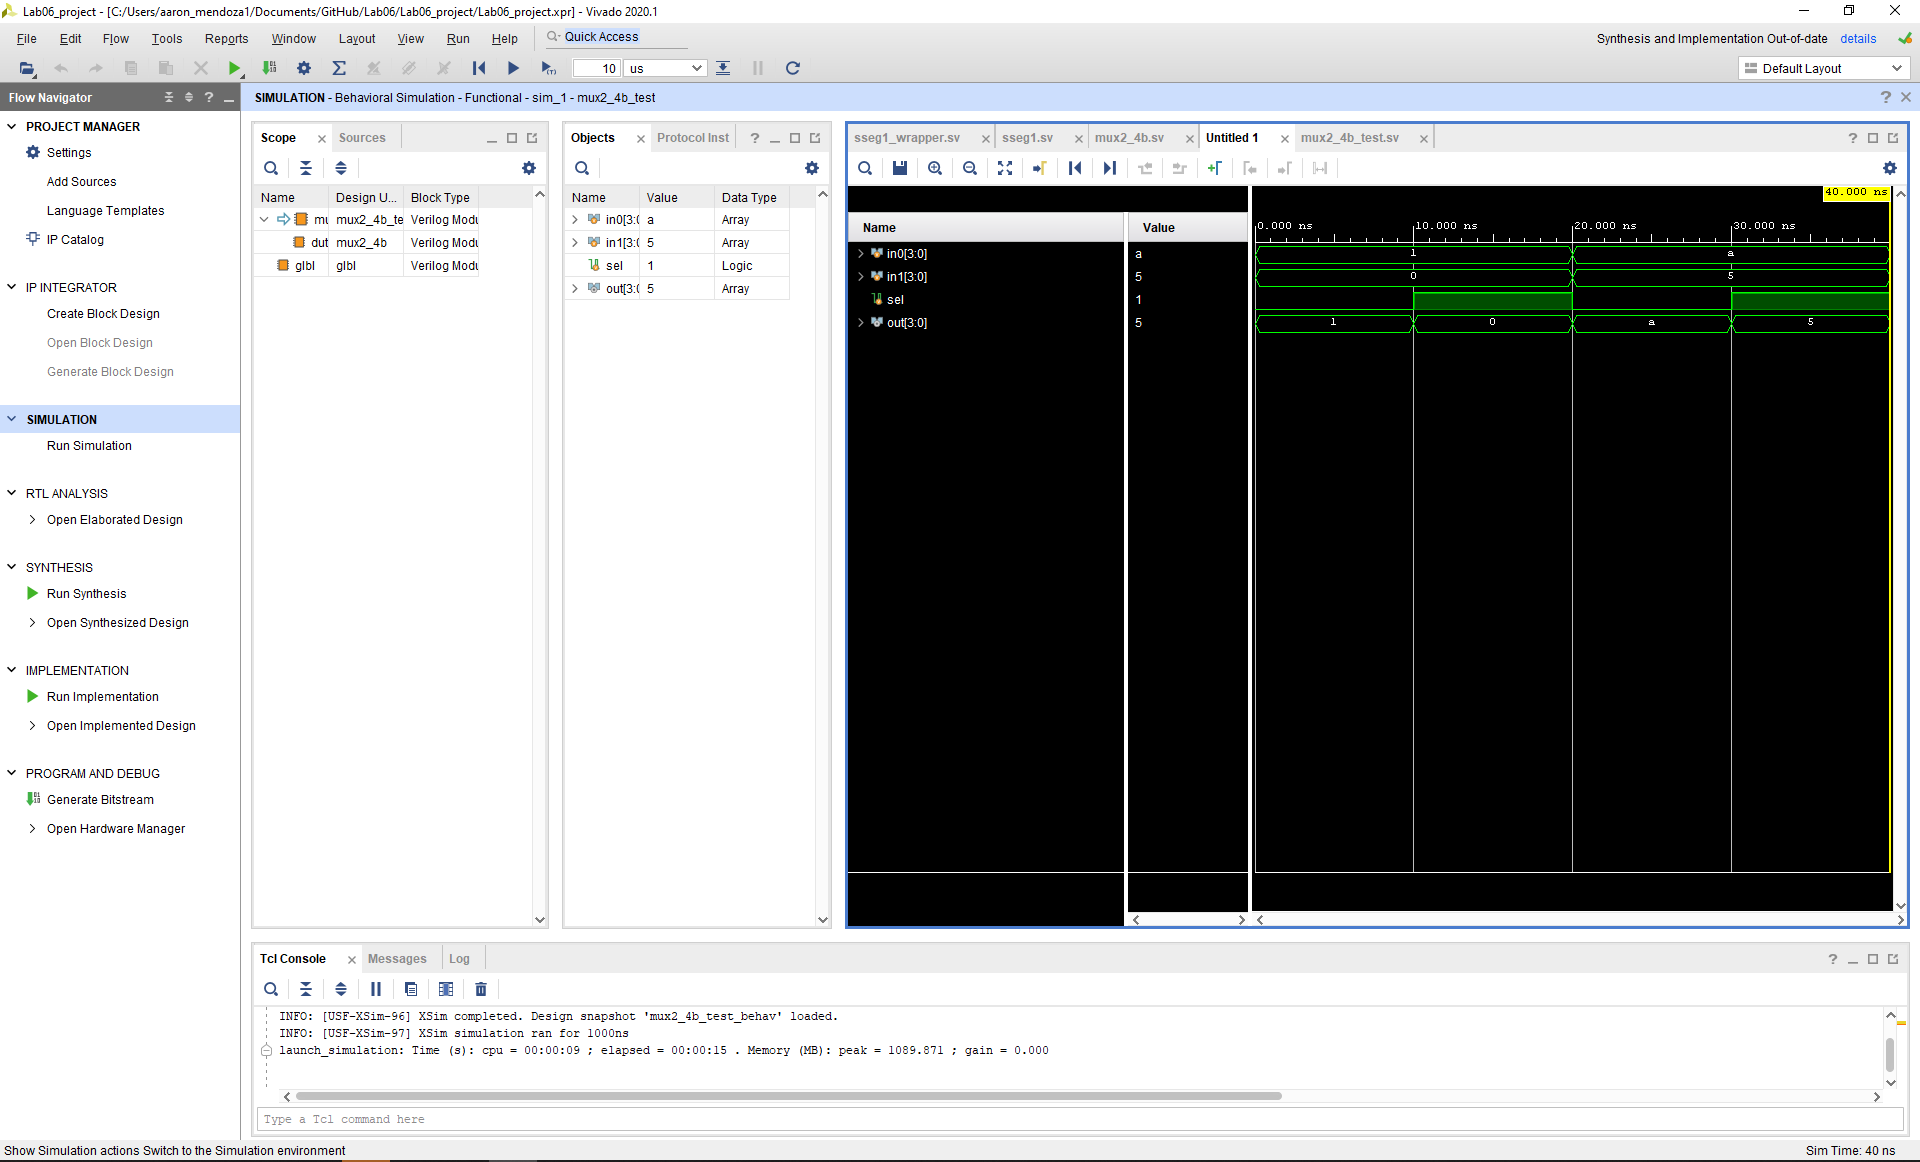
\includegraphics[width=1\textwidth,trim=21cm 18cm 0.5cm 4.7cm,clip]{mux_test_screenshot}
	\caption{MUX Simulation}
	\label{fig:sim_with_table}
\end{figure}


\begin{table}[ht]\centering
	\caption{ERT for Seven-segment Decoder}
	\label{tbl:example_table}
	\begin{tabular}{cc|cccccccccccccccc}
		\toprule
		& Time(ns) & 0 & 10 & 20 & 30 & 40 & 50 & 60 & 70 & 80 & 90 & 100 & 110 & 120 & 130 & 140 & 150 \\
		\midrule
		Input & num(hex) & 0 & 1 & 2 & 3 & 4 & 5 & 6 & 7 & 8 & 9 & A & B & C & D & E & F \\
		Output & sseg(hex)  & 0 & 1 & 2 & 3 & 4 & 5 & 6 & 7 & 8 & 9 & A & B & C & D & E & F \\
		\bottomrule
	\end{tabular} 
\end{table}

\begin{figure}[ht]\centering
	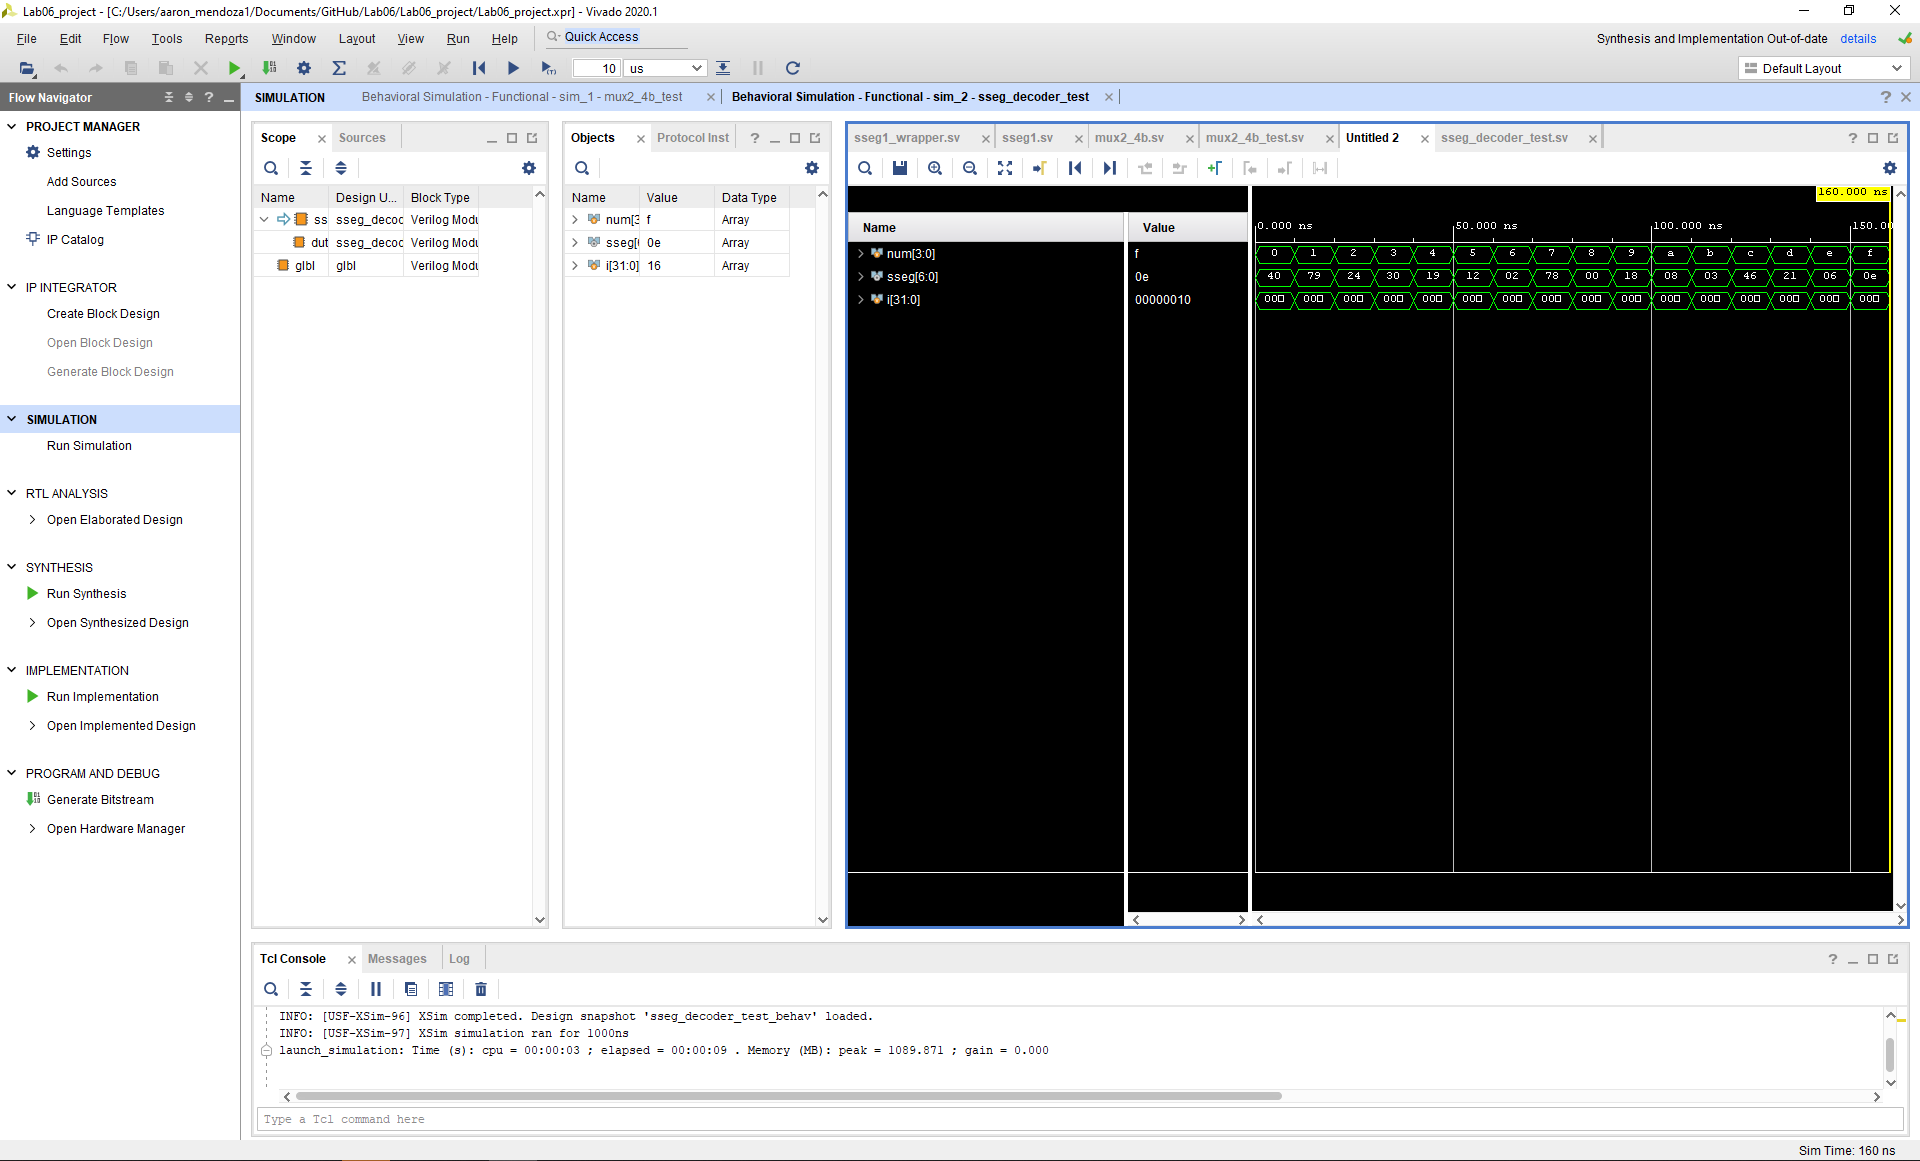
\includegraphics[width=1\textwidth,trim=21cm 18cm 0.5cm 4.7cm,clip]{sseg_decoder_screenshot}
	\caption{Decoder Simulation}
	\label{fig:sim_with_table}
\end{figure}

\begin{table}[ht]\centering
	\caption{ERT for Top-level Module}
	\label{tbl:example_table}
	\begin{tabular}{ccc|c}
		\toprule
		 A & B & sel & Output \\
		\midrule
		1010 & 0101 & 0 & 0001000 \\
		1010 & 0101 & 1 & 0010010 \\
		1001 & 0111 & 0 & 0011000 \\
		1001 & 0111 & 1 & 1111000 \\
		\bottomrule
	\end{tabular} 
\end{table}

\begin{figure}[ht]\centering
	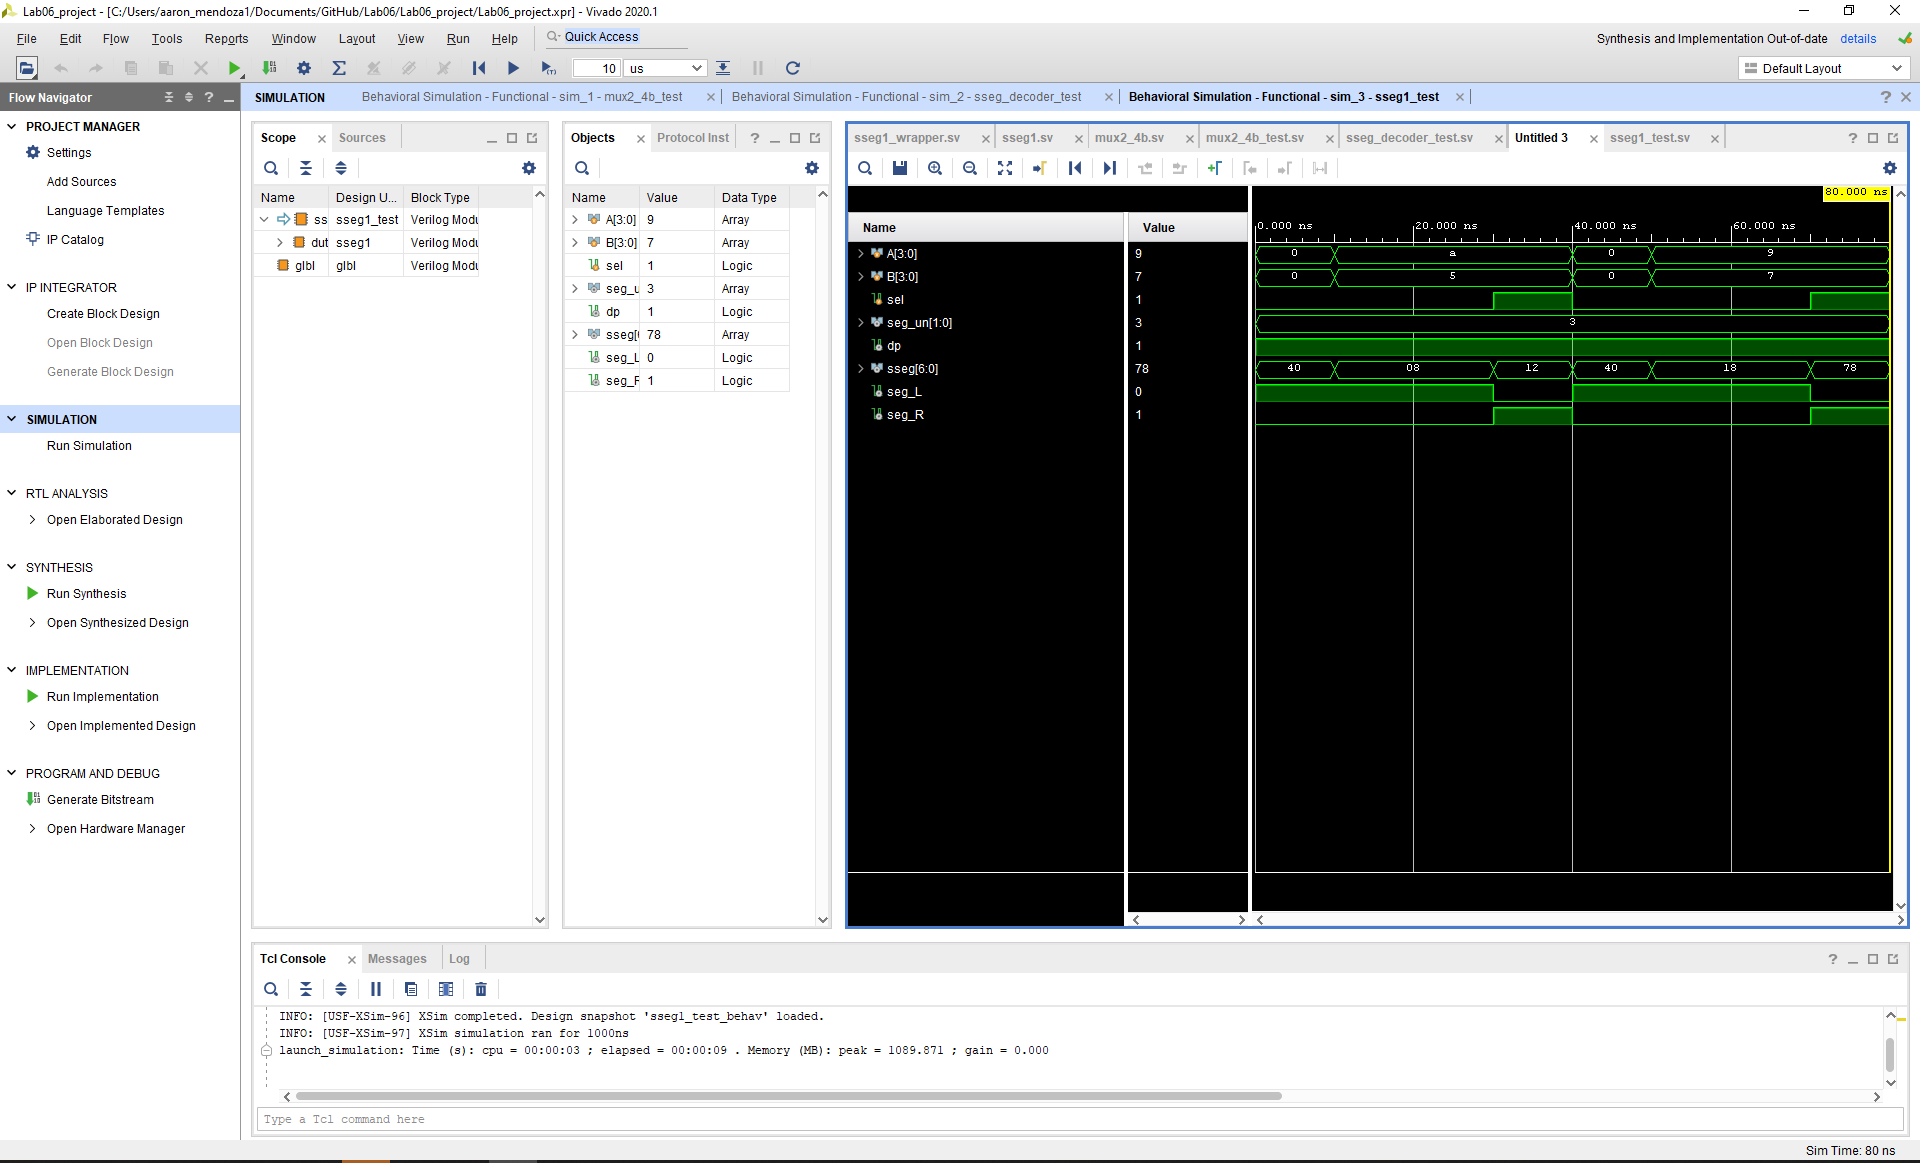
\includegraphics[width=1\textwidth,trim=21cm 18cm 0.5cm 4.7cm,clip]{sseg_screenshot}
	\caption{Top Level Simulation}
	\label{fig:sim_with_table}
\end{figure}

\begin{figure}[ht]\centering
\includegraphics[width=0.5\textwidth]{first_digit}
\caption{This is an image of the the first digit of my Basys3 board.}
\label{fig:original_logo}
\end{figure}
\begin{figure}[ht]\centering
\includegraphics[width=0.5\textwidth]{second_digit}
\caption{This is an image of the the second digit of my Basys3 board.}
\label{fig:original_logo}
\end{figure}
 \FloatBarrier
\section*{Code}

\Verilog[firstline=22, lastline=31, caption=MUX Verilog code]{Lab06_project/codedirectory/mux2_4b.sv}|

\Verilog[firstline=22, lastline=45, caption=MUX Test Verilog code]{Lab06_project/codedirectory/mux2_4b_test.sv}|

\Verilog[firstline=22, lastline=51, caption=Seven-segment Decoder Verilog code]{Lab06_project/codedirectory/sseg_decoder.sv}|

\Verilog[firstline=22, lastline=42, caption=Seven-segment Decoder Test Verilog code]{Lab06_project/codedirectory/sseg_decoder_test.sv}|

\Verilog[firstline=22, lastline=43, caption=Seven-segment Wrapper Verilog code]{Lab06_project/codedirectory/sseg1_wrapper.sv}|

\Verilog[firstline=22, lastline=53, caption=Seven-segment 1 Verilog code]{Lab06_project/codedirectory/sseg1.sv}|

\Verilog[firstline=22, lastline=57, caption=Seven-segment 1 Test Verilog code]{Lab06_project/codedirectory/sseg1_test.sv}|


\end{document}
